% chapters/hbm.tex
%
% Copyright 2022 Alexander Lyttle.
%
% This work may be distributed and/or modified under the conditions of the
% LaTeX Project Public License (LPPL) version 1.3 or later.
%
% The latest version of this license is in
% https://www.latex-project.org/lppl.txt and version 1.3 or later is part of
% all distributions of LaTeX version 2005/12/01 or later.
%
%
\chapter{Hierarchical Bayesian Models}

\todo{Introduce hierarchical models as a concept. Maybe like in Hall, start with context about generative models. Then show that when we expend models to, e.g. many stars, it is useful to extend our prior to represent correlations in the stellar population. In a sense, creating priors informed by population-level distributions. Here is a good opportunity to reference past work, and maybe expand on some of the background given in the introduction to \citep{Lyttle.Davies.ea2021}.}

\section[Stellar distances]{Distances to a stars in an open cluster}

\newcommand{\appmag}{\ensuremath{\mathrm{v}}}
\newcommand{\absmag}{\ensuremath{\mathrm{V}}}

In this section, we use the example of measuring distances to stars in an open cluster to demonstrate a hierarchical Bayesian model.

We created a set of data.

We observe the apparent visual magnitude (\(\appmag_i\)) and dimensionless parallax (\(\varpi_i\)) of \(i = 1,\dots,N_\mathrm{stars}\) stars, each at some dimensionless distance (\(d_i\)) from the observer. Each observable is measured independently with Gaussian noise characterised by \(\sigma_{\appmag,i} = 0.1\) and \(\sigma_{\varpi,i} = 0.01\) respectively.

%
\begin{equation}
    \appmag_i = \absmag_i + 5 \log_{10} d_i,
\end{equation}
%

Before introducing the model, introduce and plot the mock data and 

\subsection{Simple model}

\begin{figure}[tb]
    \centering
    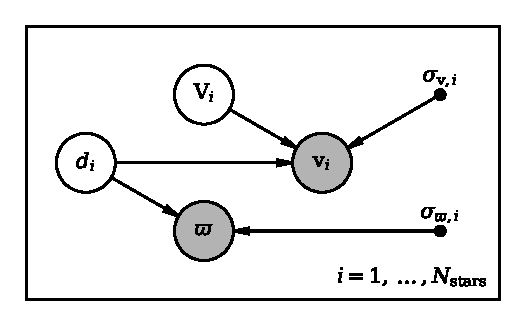
\includegraphics{figures/simple-pgm.pdf}
    \caption{Simple.}
\end{figure}

Bayes' theorem,
%
\begin{equation}
    p(d_i, \absmag_i \mid \varpi_i, \appmag_i) \propto p(\varpi_i, \appmag_i \mid d_i, \absmag_i) \, p(d_i, \absmag_i)
\end{equation}
%

We modelled the likelihood as the product of normal distributions, assuming \(\varpi_i\) and \(\appmag_i\) were observed independently,
%
\begin{equation}
    p(\varpi_i, \appmag_i \mid d_i, \absmag_i) = \mathcal{N}(\varpi_i \mid d_i^{\,-1}, \sigma_{\varpi, i}^2) \, \mathcal{N}(\appmag_i \mid \absmag_i + 5\log_{10}d_i \, , \sigma_{\appmag, i}^2).
\end{equation}
%

We assumed stars in the cluster were equally likely to be between a distance of 0 and 20. We also assumed the absolute magnitudes were likely to be normally distributed centred on 0 and scaled by 10. Therefore, the prior probability of the model parameters are,
%
\begin{equation}
    p(d_i, \absmag_i) = \mathcal{U}(d_i \mid 0, 20) \, \mathcal{N}(\absmag_i \mid 0, 100),
\end{equation}
%
where \(\mathcal{U}(x \,|\, a, b)\) is a uniform distribution over \(x\) from \(a\) to \(b\). We chose weakly-informative priors on the parameters, given that we know the true values for this example. However, these priors are fairly unrealistic and should be adapted to represent our expectation. For example, the exponential prior from \citet{Bailer-Jones.Rybizki.ea2018} would me more appropriate when observing stars radially outward from the galactic disk.

\subsection{Hierarchical model}

\begin{figure}[!tb]
    \centering
    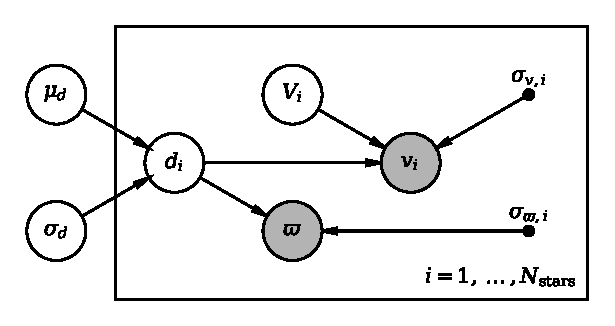
\includegraphics{figures/hbm-pgm.pdf}
    \caption{HBM.}
\end{figure}

Hierarchical,
%
\begin{equation}
    p(\mu_d, \sigma_d, \vect{d}, \vect{\absmag} \mid \vect{\varpi}, \vect{\appmag}) \propto p(\vect{\varpi}, \vect{\appmag} \mid \vect{d}, \vect{\absmag}) \, p(\vect{d} \mid \mu_d, \sigma_d) \, p(\mu_d, \sigma_d, \vect{\absmag})
\end{equation}
%

We assume \(d_i \sim \mathcal{N}(\mu_d, \sigma_d^2)\).

Maybe just do the partially-pooled case and say that the max-pooled is good when we know the parameter follows some absolute law.

\begin{figure}[p]
    \centering
    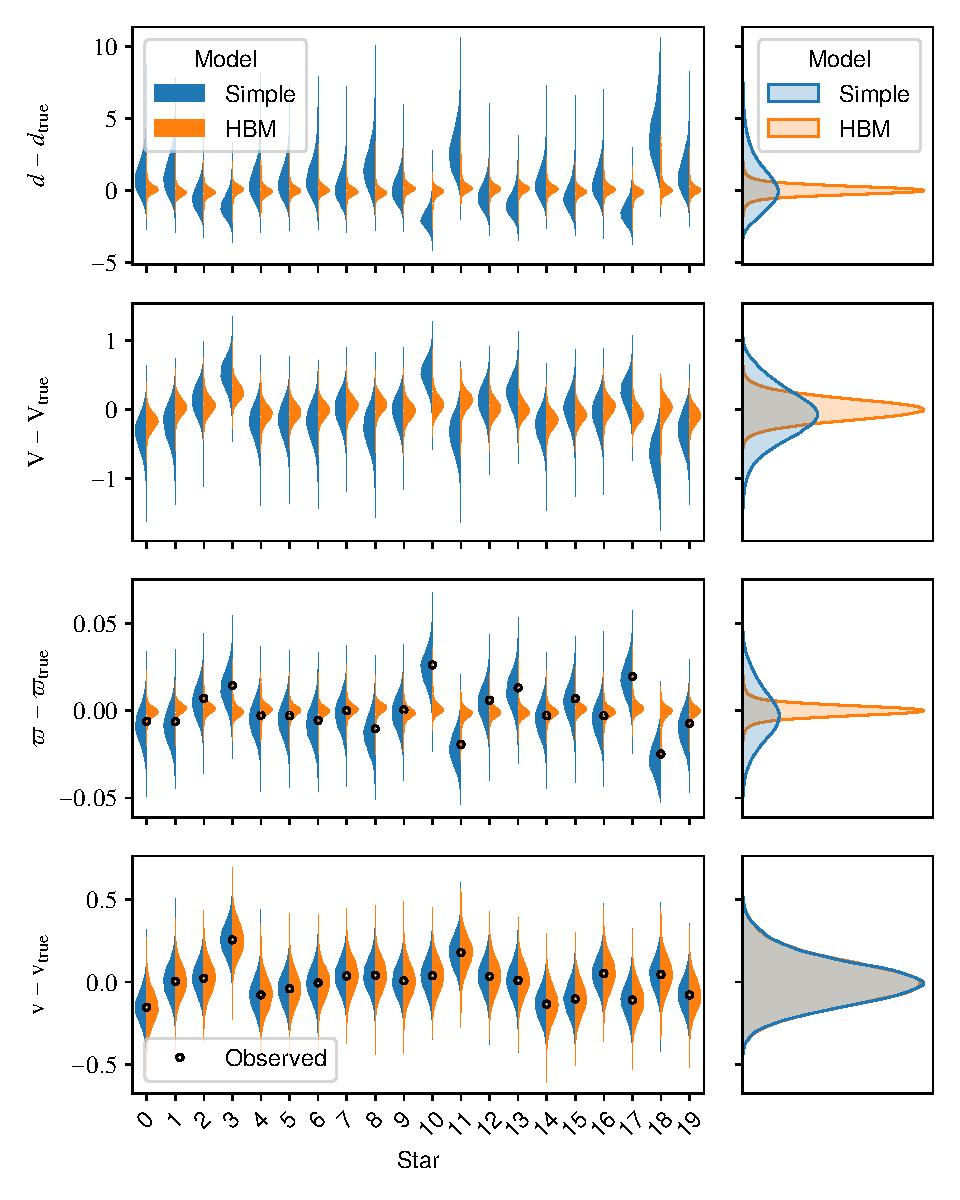
\includegraphics{figures/hbm-results.pdf}
    \caption{Results.}
\end{figure}